%%%%%%%%%%%%%%%%%%%%%%%%%%%%%%%%%%%%%%%%%%%%%%%%%%%%%%%%%%%%%%%%%%%%%%%%%%%%%%%%%%%%%%%%%%%%%%%%%%%%%%%%%%%%%%%%%%%%%%%%%%%%%%%%%%%%%%%%%%%%%%%%%%%%%%%%%%%
% This is just an example/guide for you to refer to when submitting manuscripts to Frontiers, it is not mandatory to use Frontiers .cls files nor frontiers.tex  %
% This will only generate the Manuscript, the final article will be typeset by Frontiers after acceptance.   
%                                              %
%                                                                                                                                                         %
% When submitting your files, remember to upload this *tex file, the pdf generated with it, the *bib file (if bibliography is not within the *tex) and all the figures.
%%%%%%%%%%%%%%%%%%%%%%%%%%%%%%%%%%%%%%%%%%%%%%%%%%%%%%%%%%%%%%%%%%%%%%%%%%%%%%%%%%%%%%%%%%%%%%%%%%%%%%%%%%%%%%%%%%%%%%%%%%%%%%%%%%%%%%%%%%%%%%%%%%%%%%%%%%%

%%% Version 3.4 Generated 2018/06/15 %%%
%%% You will need to have the following packages installed: datetime, fmtcount, etoolbox, fcprefix, which are normally inlcuded in WinEdt. %%%
%%% In http://www.ctan.org/ you can find the packages and how to install them, if necessary. %%%
%%%  NB logo1.jpg is required in the path in order to correctly compile front page header %%%

\documentclass[utf8]{frontiersSCNS} % for Science, Engineering and Humanities and Social Sciences articles

\usepackage{amsmath,amssymb,booktabs,url,hyperref,lineno,listings,microtype,subcaption}

% Automatic formatting of SI units
\usepackage[binary-units]{siunitx}

\usepackage[onehalfspacing]{setspace}

% Required for 'straight' quotes in code listings
\usepackage[T1]{fontenc}

% Visible TODO notes
\newcommand{\todo}[1]{\textbf{\textsc{\textcolor{red}{(TODO: #1)}}}}

\lstset{language=C++,showstringspaces=false,basicstyle=\tiny,upquote=true}

\linenumbers


% Leave a blank line between paragraphs instead of using \\


\def\keyFont{\fontsize{8}{11}\helveticabold }
\def\firstAuthorLast{Knight and Nowotny} %use et al only if is more than 1 author
\def\Authors{James C Knight\,$^{1,*}$, Thomas Nowotny\,$^{1}$}
% Affiliations should be keyed to the author's name with superscript numbers and be listed as follows: Laboratory, Institute, Department, Organization, City, State abbreviation (USA, Canada, Australia), and Country (without detailed address information such as city zip codes or street names).
% If one of the authors has a change of address, list the new address below the correspondence details using a superscript symbol and use the same symbol to indicate the author in the author list.
\def\Address{$^{1}$Centre for Computational Neuroscience and Robotics, School of Engineering and Informatics, University of Sussex, Brighton, United Kingdom }
% The Corresponding Author should be marked with an asterisk
% Provide the exact contact address (this time including street name and city zip code) and email of the corresponding author
\def\corrAuthor{James C Knight}

\def\corrEmail{J.C.Knight@sussex.ac.uk}


\begin{document}
\onecolumn
\firstpage{1}

\title[Running Title]{Article Title} 

\author[\firstAuthorLast ]{\Authors} %This field will be automatically populated
\address{} %This field will be automatically populated
\correspondance{} %This field will be automatically populated

\extraAuth{}% If there are more than 1 corresponding author, comment this line and uncomment the next one.
%\extraAuth{corresponding Author2 \\ Laboratory X2, Institute X2, Department X2, Organization X2, Street X2, City X2 , State XX2 (only USA, Canada and Australia), Zip Code2, X2 Country X2, email2@uni2.edu}


\maketitle


\begin{abstract}

%%% Leave the Abstract empty if your article does not require one, please see the Summary Table for full details.
\section{}
Inspired by the distributed nature of memory and computation in the brain, neuromorphic systems are being developed to provide a faster and/or more energy-efficient substrate for emulating spiking neural networks (SNNs) when compared to simulations running on Von Neumann architectures.

While neuromorphic systems may be the ultimate platform for \textit{deploying} spiking neural networks, their distributed nature and optimisation for specific types of models makes them unwieldy tools for \textit{developing} SNN models.
Instead development and simulation of SNN models tends to be performed on computers with standard Von Neumann CPU architectures and, once models scale above a certain size, clusters of these machines.
Over the last decade, as well as becoming a common fixture in many workstations, NVIDIA GPU accelerators have entered the High Performance Computing field and are now used in \SI{50}{\percent} of the Top 10 super computing sites to increase peak performance while lowering power requirements.
In many ways, the large amount of available parallelism and the Single Instruction Multiple Thread (SIMT) architecture of GPUs is well suited to simulating large numbers of homogeneous neurons and synapses, however it is not without challenges.
Generally, performance is good when many operations can be performed independently, for example integrating differential equations describing neuron dynamics.
When communication between threads is necessary, in particular for propagating spikes across synapses between neurons, performance can drop, in particular if connection patterns are random.
GPUs nevertheless can be very competitive for simulating SNNs with respect to speed and energy efficiency as spike events are less frequent than the time-step based updates of neuron and synapse equations that often make up the bulk of the required computation. 
\todo{argument for using GPUs for SNN -TN: I added a bit ... see whether you think it's enough}

In this paper we use our GeNN code generator to re-implement two large-scale point neuron network models with levels of connectivity and sparseness matching those in the neocortex and discuss how they are mapped to GPU hardware.
We then verify the correctness of our GPU simulations against prior results obtained with NEST on traditional HPC hardware and compare the performance with respect to speed and energy consumption against published data from CPU-based HPC and neuromorphic hardware.
We show that a full-scale model of a cortical column can be simulated at speeds approaching $0.5\times$ real-time using a single NVIDIA Tesla V100 accelerator -- faster than is currently possible using a CPU based cluster or the SpiNNaker neuromorphic system.
In addition, we find that, across a range of GPU systems, the energy to solution as well as the energy per synaptic event of the microcircuit simulation is as much as $14\times$ lower than either on SpiNNaker or in CPU-based simulations.

\tiny
 \keyFont{\section{Keywords:} GPU, high-performance computing, parallel computing, accuracy of simulation, energy to solution, benchmarking, computational neuroscience} %All article types: you may provide up to 8 keywords; at least 5 are mandatory.
\end{abstract}

\section{Introduction}
Currently, the most common way to accelerate large-scale SNN simulations is to use CPU-based HPC clusters running software simulators such as NEST~\todo{cite}, parallel Neuron~\todo{cite} or Arbor~\todo{cite}.
However spiking neural networks simulations have a large amount of \textit{fine-grained} parallelism which parallel CPU programming paradigms such as multithreading are not well-suited to exploiting.
Furthermore, although the timestep based updates of neuron and synapse dynamics are trivially parallelisable, simulating an SNN also involves the low-latency propagation of spike events between neurons along synaptic connections which is not a good match for standard interconnect technologies such as MPI.

Neuromorphic systems use dedicated hardware, inspired by aspects of the brain, to address the problems of parallelism and efficient spike communications.
The SpiNNaker system~\citep{Furber2014}, developed as part of the Human Brain project, is a neuromorphic computer consisting of up to a million ARM cores, connected with an interconnect topology optimised for spike-like communication.
Rather than using digital processors, the BrainScaleS system developed within HBP at Heidelberg~\citep{Schemmel2017}, uses analog circuit elements to emulate the dynamics if point neurons.
Spikes then propogate between these circuit elements through a digital interconnect network.
Other neuromorphic systems based a variety of combinations of digital and analog hardware include the Loihi chip~\citep{Davies2018} developed by Intel, the True North chip~\citep{Merolla2014} built by IBM and the Dynapse system~\cite{Qiao2015} developed at University of Zurich.

While neuromorphic systems offer significant theoretical advantages in terms of power efficiency and simulation speed, this often comes at the expense of flexibility.
\todo{make coherant}
In a recent publication \citet{VanAlbada2018} investigated the comparative performance of simulations of a micro-column model~\citep{Potjans2012} in NEST-based simulations on an HPC cluster and when implemented on the SpiNNaker neuromorphic system.
They found that both architectures achieved the same accuracy in simulation results when SpiNNaker was run at 20 times slower than realtime, while NEST on HPC achieved 3 times slower than realtime. 
The lowest energy consumption for NEST was achieved with 144 parallel threads when it ran at 4.6 times slower than realtime. 
At this speed SpiNNaker and NEST and SpiNNaker consumed about the same energy \SI{6}{\micro\joule} per simulated synaptic event.

\todo{We need to make some statements about how network creation and
  initialisation are a problem that has been identified only recently
  to have major impacts on runtime and energy efficiency (and cite
  Diamond 2016 paper). Maybe here. I think this paper is as much about your new
  parallel init stuff as about beating SpiNNaker and NEST ... ?}

\todo{make coherant}
Additionally, while a lack of global synchronisation is indeed biomimetic and makes very large-scale distributed systems like SpiNNaker possible, it makes traditional debugging techniques impossible \todo{is debugging relevant to this paper? feels like a loose end} a
\todo{FPGA}
Alternatively, GPU architectures are specifically designed for high throughput applications with large amounts of fine-grained paralelism.
They sacrifice the large coherant caches that modern CPU architectures rely upon to improve performance for high-perforamance
The SIMT programming model architecture used by NVIDIA GPUs is designed explicitly for fine-grained parallelism and high throughput.
\todo{make coherant}
%At this step, computations need to be synchronised and clever update algorithms are required to make use of parallelization while at the same time avoiding conflicts in memory access, e.g. when spikes from different neurons arrive at the same post-synaptic site.
As such, there is a number of active SNN simulator projects that are tergetting GPUs. Carlsim~\citep{Chou2018} is a C++ based simulator runnning on NVIDIA CUDA with similar goals as GeNN but is not based on code generation and hence less flexible in the types of models it can support.
EDLUT~\citep{Garrido2011} was initially an event drive CPU based simulator for SNNs but now has become a hybrid CPU/GPU system with a timestep based GPU accelerator.
ANNarchy~\citep{Vitay2015} is a code generation based simulator translating Python models descriptions into multi-core CPU or GPU code with a focus on hybrid rate- and spiking models.
Other simulators that have seen less development in the last 2-4 years include NCS6~\citep{Hoang2013}, Myriad~\citep{Rittner2016}, and NeMo~\citep{Fidjeland2009} (see \citet{Brette2012} for a review).
\todo{something about GeNN}

In this paper we introduce novel methods for parallel initialisation of neuronal network models in our GeNN simulator and investigate the performance of a GPU based simulation in GeNN of the micro-column network model \cite{Potjans2012,vanAlbada2018} as well as a model using STDP in a highly connected network~\citep{Morrison2007} to competitively benchmark a GPU based solution for SNN simulations.

\section{Material and Methods}
\label{sec:method}
\subsection{GeNN}
\label{sec:method/genn}
\todo{Make coherant}A different kind of challenge comes from the rapidly developing GPU hardware which necessitates specific optimisations for each specific GPU architecture.
Many aspects of this are being taken care of by the Compute Unified Device Architecture (CUDA) application programming interface and nvcc compiler developed by NVIDIA Corporation.
CUDA offers an abstraction layer that allows programmers to work in a common programming model of threads, warps and blocks across generations of CUDA enabled devices.
However, some details such as parallelisation strategies, block sizes and memory access patterns remain to be optimised for each device by the programmer.
As described elsewhere~\cite{Yavuz2016}, GeNN solves these complications using a code generation system that lets users define SNNs and their dynamics in abstract form and takes care of the underlying CUDA programming.

GeNN neuron models are defined by writing a class defining the model parameters and snippets of C-like code that describe how it should be simulated.
For example the following \lstinline{LIF} class describes a leaky integrate-and-fire neuron with normalised units, solved algebraically:

\lstinputlisting[firstline=2,lastline=15]{code_snippets.cc}

The \lstinline{DECLARE_MODEL} and \lstinline{IMPLEMENT_MODEL} macros insert boilerplate code used subsequently for defining parameters and initial model states in a type-safe manner.
The \lstinline{SET_SIM_CODE}, \lstinline{SET_THRESHOLD_CONDITION_CODE} and \lstinline{SET_RESET_CODE} macros specify the snippets of code used, respectively, to update the simulation state, check whether a spike should be emitted and to reset the neuron after a spike.
The names of model parameters (constant across the entire population) are specified using the \lstinline{SET_PARAM_NAMES} macro and any `pre-processing' logic to be applied to these is specified with \lstinline{SET_DERIVED_PARAMS} -- in this case converting an exponential decay time constant to a multiplier to be applied every simulation timestep.
Finally, the \lstinline{SET_VARS} macro specifies the names and types of the per-neuron state variables.
These macros provide some `syntactic sugar' but are entirely optional -- users can instead override the underlying virtual functions themselves.
In GeNN synapse models are defined using very similar classes with the option to define code snippets for time-driven and event-driven updates.
Event-driven updates can be triggered by pre or postsynaptic spikes as well as by custom events for example the pre or postsynaptic neuron's membrane voltages crossing a threshold.
Once the required models have been defined, the values of parameters and initial state variables can be set and \textit{populations} of neurons can be added to a network:
%
\lstinputlisting[firstline=17,lastline=20]{code_snippets.cc}

\todo{we need to say somewhere that this is new ... maybe in the introduction}This listing also illustrates how the approach used for defining models can also be used to define how variables are initialised.
The membrane voltage \lstinline{V} of our \num{1000} LIF neurons is sampled from the uniform distribution using one of GeNN's built in \textit{variable initialisation snippets}.
These are definied in a similar manner to the neuron and synapse models previously described, allowing network initialisation to be parallelised using the same strategies used for simulating models on the GPU for initialising their parameters.
This approach is advantageous as it both removes the need to transfer the model state from the CPU to the GPU and it allows the GPU to be used to accelerate potentially costly initialisation operations such as sampling random numbers.
%While the PCI express bus typically used to connect the GPU to the host system is relatively fast (up to \SI{16}{\giga\byte\per\second}), initialising millions of synaptic weights on the CPU and then uploading them at the start of the simulation can still considerably slow down the time it takes to iterate the model.

Once network models have been defined using the C++ interface described in the preceding section, GeNN will generate the CUDA code to simulate the network and this can be linked against a simple simulation loop provided by the user:

\lstinputlisting[firstline=22,lastline=32]{code_snippets.cc}

While this approach allows a lot of flexibility and means that visualisation tools and closed-loop robotics can be tightly coupled to GeNN simulations, when combined with the use of C++ for model definition, this does make using GeNN a somewhat daunting prospect to users more used to Python-based simulations such as Brian~\citep{Stimberg2014} or PyNN~\citep{Davison2008a} or graphical tools such as SpineCreator~\cite{}.
For these users GeNN can be used as a backend for other other simulators.
Brian2GeNN~\citep{Stimberg2018} allows models to be defined in Brian 2 and translates them using code generation into a valid GeNN simulation. 
Using Brian 2's backend device design, using GeNN through Brian2GeNN is as simple as issuing the command \lstinline[language=python]{set_device("brian2genn")} within a standard Brian 2 script. 
A similar interface exist for SpineML~\citep{Richmond2014} and an interface to PyNN~\citep{Davison2008a} is currently being developed.

\subsection{The cell-type specific cortical microcircuit}
\label{sec:method/microcircuit}
This model of \SI{1}{\milli\metre\cubed} of early-sensory cortex was first developed by \citet{Potjans2012}.
The model consists of around \num{80000} neurons, divided into layers 2/3, 4, 5 and 6 and each layer is modelled as an excitatory and an inhibitory population.
Neurons in each population are connected with population-specific densities derived from an extensive review of the anatomical literature resulting in a total of approximately \num{0.3E9} synapses.
The connections between a presynaptic population with $N_{pre}$ neurons and a postsynaptic population with $N_{post}$ neurons are specified as a total number of randomly-distributed synapses (a \lstinline{FixedNumberTotal} connector in PyNN).
The first stage in initialising such connectivity is to determine how many of the total synapses $N$ end up in each row by sampling from the multinomial distribution $Mult[N_{pre} * N_{post}, \{P_{row}, P_{row}, \ldots, P_{row}\}]$ where $P_{row} = \frac{N_{post}}{N}$.
This operation cannot be efficiently parallelised so must be performed on the host but, once the length of each row is determined, the postsynaptic targets of the synapses can be initialised in parallel by sampling from the discrete uniform distribution $Unif[0, N_{post}]$ parallelised across $N_{pre}$ CUDA threads.
However, although this works mathematically, so as to improve the locality of memory accesses, synapses should be sorted into ascending order.
This would be trivial to implement in CPU code but, without enough shared memory for each CUDA thread to store a copy of its corresponding row, an in-place sort in global memory would be very slow.
It would be possible to use a more complex parallel sorting algorithm such as that proposed by \citet{Awan2016} but, as GPU architectures typically have very high floating point maths throughput, we instead take an alternative approach.
Rather than sampling directly from $Unif[0, N_{post}]$ we sample from its 1st order statistic $Beta[1, N_{post}]$ -- essentially the next smallest value.
In the general case the Beta distribution cannot be sampled from in constant time.
However, if $X \sim Beta[1, N_{post}]$, $1 - X \sim Beta[N_{post}, 1]$ and $-ln(1 - X) \sim Exponential[N_{post}]$ -- a much simpler problem as the exponential distribution can be sampled in constant time using the inversion method.

Beside this structured connectivity, all synaptic strengths and transmission delays are normally distributed.
\todo{Thomas: is it necessary to go into further details of network structure or just refer reader to Potjans2012? - TN: I think we should not go deeper into this and refer to the Potjans paper}
In addition to their synaptic input, each neuron in the network also receives independent Poisson inputs with population-specific rates representing input from adjacent cortical regions.
Neurons are modelled as leaky integrate-and-fire~(LIF) units with exponentially shaped current inputs:
%
\begin{align}
    \tau_{m} \frac{dV_{j}}{dt} = & (V_{j} - V_{rest}) + R_{m}(I_{bias} + I_{s_{j}}) \label{eq:lif_neuron}\\
    \tau_{syn} \frac{dI_{s_{j}}}{dt} = & -I_{s_{j}} + \sum_{i=0}^{n} w_{ij} \sum_{t_{i}^{f}}  \delta(t - t_{i}^{f})\label{eq:exp_neuron_input_current}
\end{align}
%
Although $V_{j}$ and $I_{s{j}}$ are coupled, in our GeNN model, the continuous terms of the two equations are solved separately so the synaptic input current $I_{s_{j}}$ going into equation~\ref{eq:lif_neuron} is effectively treated as a constant during each simulation timestep.
As \citet{Rotter1999} describes, this approach leads to a delay of one simulation timestep compared to the exact solution, but this separation is not only attractive from an engineering point-of-view by better encapsulating the neurons and synapses, but it also provides a generic way of describing neurons with heterogeneous synaptic input dynamics.

Simulating a homogeneous \textit{population} of neurons is an ideal task for a SIMD or SIMT device such as a GPU: the neurons do not communicate with each other and, aside from the relatively rare times that they spike, each neuron will be running exactly the same code.
This means that they can be trivially parallelised by simulating each neuron on a single thread which fetches the neuron's state variables from global memory into registers at the start of each timestep, then advances the simulation state and writes back the state variables.
As long as the state variables are laid out correctly in memory, the required memory operations can be \textit{coalesced} so that a \SI{4}{\byte} state variable can be read for \num{32} neurons in a single \SI{128}{\byte} transaction -- the most efficient way to access the global memory.
%This same parallelism strategy is equally valid for neuron models whose dynamics can only be solved numerically -- the advancing of simulation state simply has to be implemented as for example a Runge-Kutta

\begin{figure}
    \begin{center}
        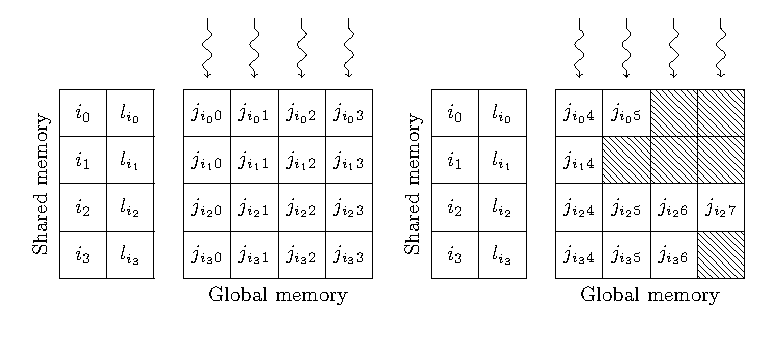
\includegraphics[width=118mm]{figures/ragged_matrix}
    \end{center}
    \caption{GPU parallelism of sparse synaptic matrix processing across two thread blocks each with \num{4} threads.
    Snaking lines indicate CUDA threads.
    Hatching indicates padding entries.}
    \label{fig:ragged_matrix}
\end{figure}

Simulating the sparsely connected synapses between two such populations of neurons is, at first glance, less suitable for GPU parallelism.
However, on modern GPU hardware, this can also be implemented in an efficient manner using the data structures shown in figure~\ref{fig:ragged_matrix}.
This structure consits of multiple 2D arrays where each row represents the synapses coming from a single presynaptic neuron and has enough columns to contain the largest number of postsynaptic targets any presynaptic neuron connects to.
One of these 2D arrays is used to contain the indices of the postsynaptic neurons ($i$) and additional arrays are allocated for any individual synaptic state variables such as the synaptic weight~($w_{ij}$) or dendritic delay~($d_{ij}$).
Each block of $N_{block}$ CUDA threads (in figure~\ref{fig:ragged_matrix} $N_{block}=4$) is responsible for processing $N_{block}$ columns of the matrix.
Processing begins by using the $N_{block}$ thread to fetch the indices of $N_{block}$ presynaptic spikes ($i_{0},\ldots,i_{N_{block} - 1}$) and the lengths of the corresponding rows of the matrix ($l_{0},\ldots,l_{N_{block} - 1}$) into shared memory (as these will be accessed by all threads in the block during the next phase).
Threads are then synchronised and loop through the $N_{block}$ rows with each thread processing the synapse in their column.
In the case of the simple static synapses described by equation~\ref{eq:exp_neuron_input_current} this processing consists simply of reading the index of the postsynaptic target neuron along with the weight $w_{ij}$ and delay $d_{ij}$ associated with the connection and using an atomic add operation to apply the weight to the correct address in the dendritic delay ring-buffer.\todo{say more}
This process is then repeated until all incoming spikes are processed.
While this parallelism strategy may seem counter-intuitive, it typically performs much better than the naïve approach of using one thread per incoming spike as it exposes much more parallelism as well as resulting in perfectly coalesced memory read operations.
For example, if we consider a population of \num{10000} neurons firing at an average rate of \SI{10}{\hertz}, in a \SI{0.1}{\milli\second} timestep it will only, on average, emit \num{10} spikes in a single timestep.
However, if this population is connected to another population with the same size with a \SI{10}{\percent} connection probability, the connection matrix will have over \num{1000} columns resulting in 2 orders of magnitude more parallelism being exposed.

\subsection{Balanced random network with spike-timing dependant plasticity}
\label{sec:method/balanced_random}
The type of one-shot, online learning observed in nature is one of the features of biological neural networks that neuromorphic engineers aspire to emulate.
Synaptic plasticity -- the family of mechanisms responsible for changing the strength of synaptic connections in response to neural activity -- has been shown to be fundamental to learning~\citep{Nabavi2014} and is therefore a key area of computational neuroscience research.
Spike Timing Dependant Plasticity~(STDP)~\citep{Bi1998} is a popular theory which postulates that these changes are driven by the difference in timing between presynaptic spikes arriving at a synapse and the times at which the postsynaptic neuron itself spikes.
In excitatory cortical neurons~\citep{Markram1997} as well as in the Hippocampus~\citep{Bi1998}, synapses at which a presynaptic spike is closely followed by a postsynaptic spike are strengthened whereas those at which a postsynaptic spike precedes a presynaptic spike are weakened.
The intuition behind this relationship is that synapses that are implicated in the firing of the postsynaptic neuron are strengthened and those that are irrelevant are weakened.

However, adding STDP to spiking neural network simulations typically increases the computational cost of simulating them significantly. 
\citet{Morrison2007} reported that adding plasticity to their simulations slowed them down by ``a factor of less than 10'' and \citet{Knight2016b} found that, in the \textbf{best} case, simple STDP plasticity reduced the performance of the SpiNNaker neuromorphic system by approximately $6\times$.
Furthermore, the dynamics of neural systems with plasticity operating on biologically-plausible time scales also take several orders of magnitude more time to stabilise.
%Perhaps because of these issues, there are relatively few large-scale network models with synaptic plasticity.
However, \citeauthor{Morrison2007} argue that it is vital to perform experiments on STDP in models with full-scale connectivity, as simplifying connectivity typically results in fewer, stronger incoming synapses per neuron.
These stronger synaptic inputs are then likely to increase the correlation between neurons and, because STDP is inherently sensitive to correlated neural activity, this is likely to cause artefacts in the learned synaptic weights.
Therefore \citeauthor{Morrison2007} developed a large balanced random network model~\citep{Brunel2000} with \num{90000} excitatory and \num{22500} inhibitory neurons -- the scale necessary to achieve realistic connection probabilities of $\approx0.1$ and \num{10000} incoming connections per neuron~\citep{braitenberg2013cortex}.
Balanced random networks have been shown to reproduce some of the dynamics seen in the neocortex~\citep{Brunel1999,Brunel2000} and \citeauthor{Morrison2007} showed that adding STDP to such a network does not disrupt these dynamics and that weights remain stable.

Similarly to the microcircuit model described in the previous section this model uses LIF neurons with current inputs.
However, rather than exponentially filtering the incoming synaptic input, this model uses a slightly more complex \textit{alpha} synapses \todo{cite} which provide a closer match to the dynamics of biological ion channels:
%
\begin{align}
    \tau_{syn} \frac{dI_{s_{j}}}{dt} = & x_{s_{j}} - I_{s_{j}} \label{eq:alpha_neuron_input_current_1}\\ 
    \tau_{syn} \frac{dx_{s_{j}}}{dt} = & -x_{s_{j}} + \sum_{i=0}^{n} w_{ij} \sum_{t_{i}^{f}}  \delta(t - t_{i}^{f}) \label{eq:alpha_neuron_input_current_2}
\end{align}
%
Aside from requiring an additional state variable to hold $x_{s_{j}}$, equations~\ref{eq:alpha_neuron_input_current_1}~and~\ref{eq:alpha_neuron_input_current_2} are i
As well as alternative synaptic plasticity rules which use postsynaptic membrane voltage~\citep{Brader2007,Clopath2010c} rather than postsynaptic spike times and those including `third factors' such as dopamine~\citep{Izhikevich2007}, there are a plethora of different STDP formalisations (see \citet{Morrison2008} for a review).
However, in the model described in this section, \citet{Morrison2007} chose to use a rule with the following relationship between pre~($t_{pre}$) and postsynaptic~($t_{post}$) spike timing ($\Delta t = t_{post} - t_{pre}$):
%
\begin{align}
    \Delta w_{ij} & = \
        \begin{cases}
            \lambda w_{0}^{1-\mu} w_{ij}^{\mu} e^{-\frac{|\Delta t|}{\tau}} & if\, \Delta t>0\\
            -\lambda \alpha w_{ij} e^{-\frac{|\Delta t|}{\tau}}             & if\, \Delta t\leq0
        \end{cases}
\end{align}
%
This rule can be implemented 

\begin{figure}
    \begin{center}
        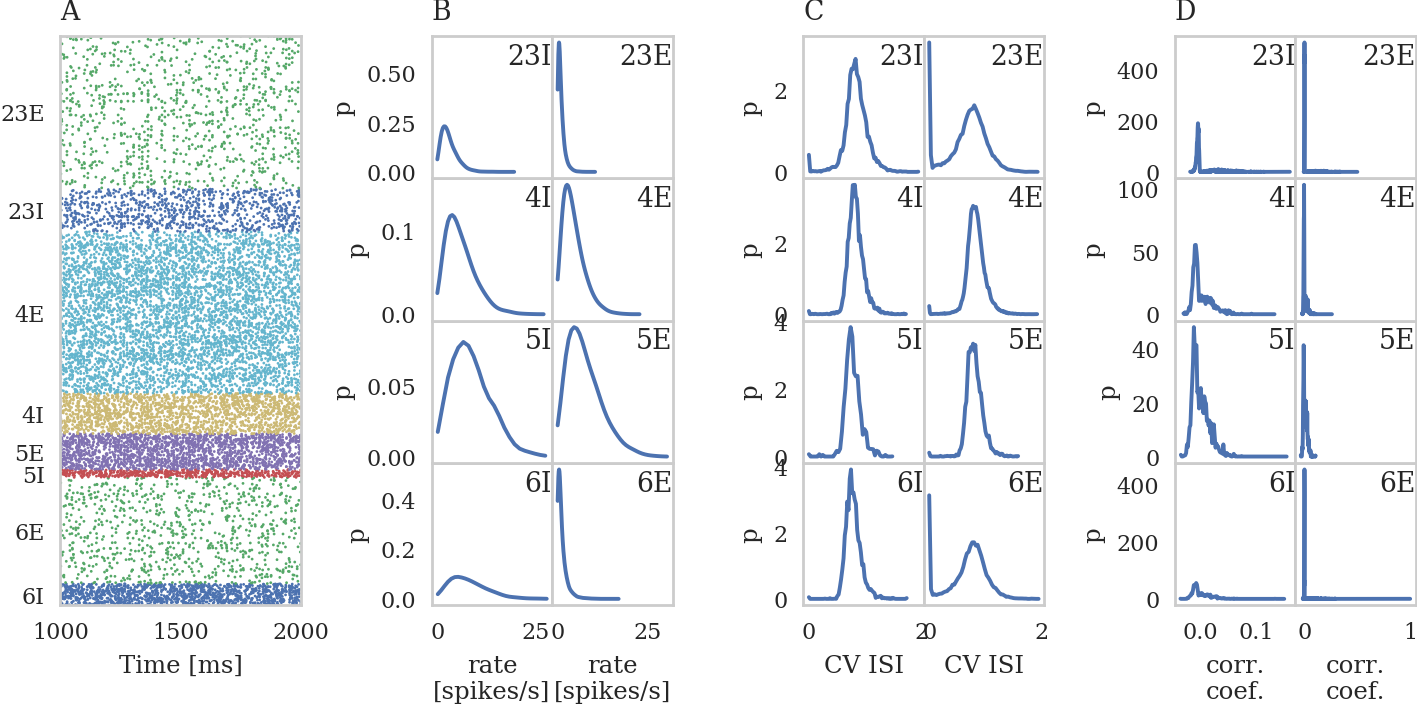
\includegraphics[width=180mm]{figures/microcircuit_accuracy}
    \end{center}
    \caption{Spiking output of cortical microcircuit model with Poisson input.\\
    \textbf{(A)} Raster plot showing spike times (dots) of neurons from each population.
    The spikes of 5\% of neurons (vertical) are shown.\\
    \textbf{(B)} Single-neuron firing rates of all neurons.\\
    \textbf{(C)} CV ISI, a measure of irregularity of all neurons.\\
    \textbf{(D)} Correlation coefficients between binned spike trains for \num{200} neurons in each population.
    All measures are calculated over the last \SI{9}{\second} of the simulation and histogram bin widths are determined using the Freedman-Diaconis rule.}
    \label{fig:microcircuit_accuracy}
\end{figure}

\section{Results}
\subsection{Correctness}
\label{sec:results/correctness}
\citet{VanAlbada2018} performed an in-depth analysis of the correctness of simulations of the microcircuit model described in section~\ref{sec:method/microcircuit} running on both the SpiNNaker neuromorphic system and NEST running in `grid-based' mode.
While the GPU simulations presented in this paper do not face the issues with quantisation which can affect SpiNNaker, unlike NEST, they all use single rather than the double-precision floating point and therefore have the potential for more numerical instability.
Additionally, the non-associative nature of floating point operations mean that, if the results from a large number of parallel threads are summed together in a non-deterministic order, can have large error bounds.
\citet{Villa2009} demonstrated this by calculating the Euclidian sum of \num{28000} double-precision floating point numbers across \num{16000} threads of a CRAY XMT system (which, in this context, has similar properties to a GPU) and found that results varied by up to \SI{24.64}{\percent}.
However, in this experiment, more numbers were summed than occurs in any of the parallelism schemes described in section~\ref{sec:method} and it is unclear what absolute errors these reported relative errors correspond to.
Nonetheless, in this section we will confirm the correctness of our simulations using the methodology described by \citet{VanAlbada2018} to compare the results of our microcircuit simulation to those computed using NEST running in `precise' mode.

While the randomisation of each neurons initial membrane voltage should reduce any such effects, the first \SI{1}{\second} of spike data from each \SI{10}{\second} simulation is discarded in order to remove any transients.
We then calculated the average firing rates and the covariance of interspike interval~(CV ISI) for each neuron in the model throughout the remaining \SI{9}{\second} of spiking data using the Elephant~\citep{Yegenoglu2018} package.
We also picked \num{200} (this was a tradeoff between accuracy and analysis time chosen by \citeauthor{VanAlbada2018}) active neurons from each population, binned their spike trains into \SI{2}{\milli\second} bins (corresponding to the refractory time of the neurons) and calculated the Pearson correlation coefficients matrix between each disjoint pair of neurons.

The same statistics were then calculated from a NEST simulation running in `precise' mode.
Histograms of all three measures were then produced using bins calculated with the Freedman-Diaconis rule~\citep{Freedman1981} from the NEST data.
These histograms were then smoothed using a Gaussian kernel density estimation performed using the \lstinline{scipy.stats.gaussian_kde} function with the bandwidths of \SI{0.3}{\per\second}, \num{0.04} and \num{0.002} for the average firing rates, the CV ISI and the correlation respectively.

Figure~\ref{fig:microcircuit_accuracy} shows the results of this analysis.
Visually it is clear that the per-population distributions are highly similar and, to quantify this, we calculated the Kullback-Leibler~(KL) divergences using the NEST data as a reference.
As reported by \citet{VanAlbada2018} for their grid-aligned NEST and SpiNNaker simulations, the divergence between the distributions from the GeNN simulations and those produced by NEST running in `precise' mode are comparable in size to the divergences caused by simply changing the seed used for random number generation.
This suggests that using single-precision floating point and summing inputs in a non-deterministic order has a minimal effect on the dynamics of the microcircuit model.

Additionally we will compare the results of simulations of the balanced random network model we describe in section~\ref{sec:method/balanced_random} with those presented by \citet{Morrison2007}.

\subsection{Performance}
\label{sec:results/performance}
To assess the performance of our GPU simulations we chose the selection of GPUs listed in table~\ref{tab:gpu_devices} -- covering a range of financial and power budgets.
CUDA abstracts away the degree of parallelism exposed by the application from the amount of hardware parallelism available so we can run a model that uses \num{80000} threads on a GPU with many fewer CUDA cores.
However memory is a harder constraint and, because of this, while all of the GPUs listed in table~\ref{tab:gpu_devices} can run the microcircuit model described in section~\ref{sec:method/microcircuit}, only the two `Tesla' GPUs have enough memory to run the balanced random network model described in section~\ref{sec:method/balanced_random}.

\begin{table}
  \centering
  \begin{tabular}{r S r S S S S}
    \toprule
        {Model}         & {TDP}             & {Architecture}    & {Num.}    & {Memory}              & {Memory}                      & {Max single-precision}\\
                        & {[\si{\watt}]}    &                   & {CUDA}    & {capacity}            & {bandwidth}                   & {performance}\\
                        &                   &                   & {cores}   & {[\si{\giga\byte}]}   & {[\si{\giga\byte\per\second}]}& {[GFLOPS]}\\
    \midrule
        GeForce 1050 Ti & 75                & Pascal            & 768       & 4                     & 112                           & 2100\\
        Jetson TX2      & 15                & Pascal            & 256       & 4\textsuperscript{1}  & 58.4                          & 600??\\
        Tesla K40c      & 235               & Kepler            & 2880      & 12                    & 288                           & 4290\\
        Tesla V100      & 250               & Volta             & 5120      & 16                    & 900                           & 14000\\
    \bottomrule
  \end{tabular}

  \caption{GPU devices.\\
  \textsuperscript{1}~Memory is shared between CPU and GPU.}
  \label{tab:gpu_devices}
\end{table}

\begin{figure}
    \begin{center}
        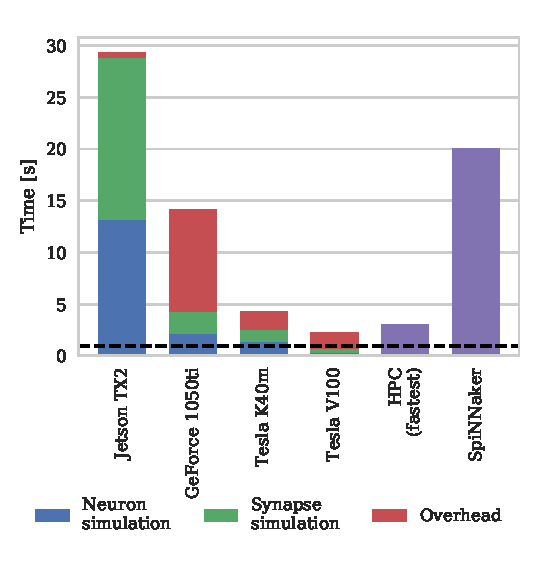
\includegraphics[width=85mm]{figures/microcircuit_performance}
    \end{center}
    \caption{Simulation times of microcircuit model running on various GPU hardware for \SI{10}{\second} of biological time.
    SpiNNaker and fastest HPC simulation times (12 nodes) presented by \citet{VanAlbada2018} included for comparison.
    `Overhead' in GPU simulations refers to time spent in simulation loop but not within CUDA kernels.}
    \label{fig:microcircuit_performance}
\end{figure}

\begin{figure}
    \begin{center}
        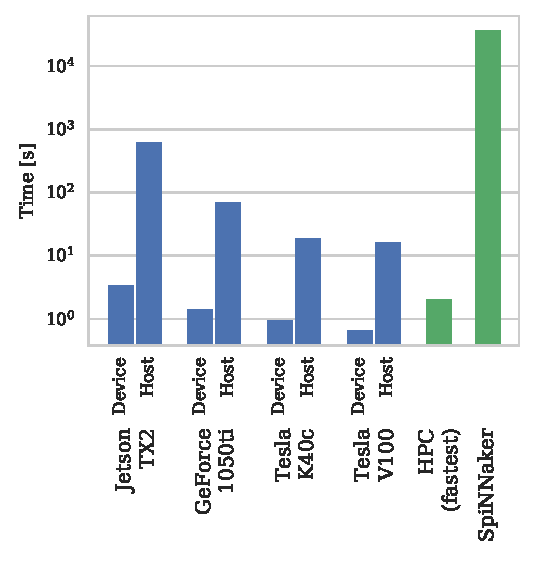
\includegraphics[width=85mm]{figures/microcircuit_init_performance}
    \end{center}
    \caption{Initialisation times of microcircuit model running on various GPU hardware.
    SpiNNaker and fastest HPC simulation times (32 nodes) presented by \citet{VanAlbada2018} included for comparison.}
    \label{fig:microcircuit_init_performance}
\end{figure}

We measured the performance of both models by querying the \lstinline{std::chrono::high_resolution_clock} on the host computer around the simulation loop to get a total simulation time and, in the case of the microcircuit model, around the code used to calculate the connectivity.
Additionally we used CUDA's own event timing system~\citep[Section~8.1.2]{NVIDIACorporation2018} to record the time taken by the neuron and synapse simulation kernels as well as the postsynaptic learning kernel in the balanced random network model.

Figure~\ref{fig:microcircuit_performance} shows the durations of simulations of the microcircuit model running on each GPU for \SI{10}{\second} of biological time, including the times taken by neuron and synapse simulation kernels.


As discussed in section~\ref{sec:method/genn}, as well as parallelising neuron and synapse simulation code, GeNN can also parallise the initialisation of model state variables and connectivity.
Figure~\ref{fig:microcircuit_init_performance} shows the initialisation time of the microcircuit simulation 

\begin{figure}
    \begin{center}
        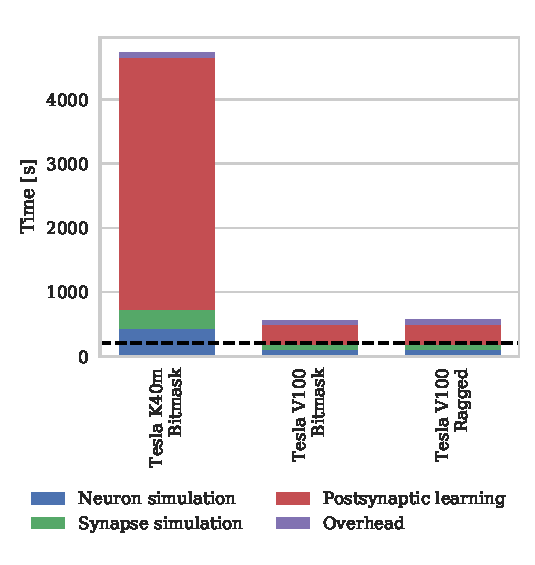
\includegraphics[width=85mm]{figures/stdp_performance}
    \end{center}
    \caption{Simulation times of balanced random network model running on various GPU hardware for \SI{200}{\second} of biological time.
    `Overhead' in GPU simulations refers to time spent in simulation loop but not within CUDA kernels.}
    \label{fig:stdp_performance}
\end{figure}

\todo{volta `Independent Thread Scheduling' may be part of the reason why second model works so well}

\subsection{Power and energy}

\begin{figure}
    \begin{center}
        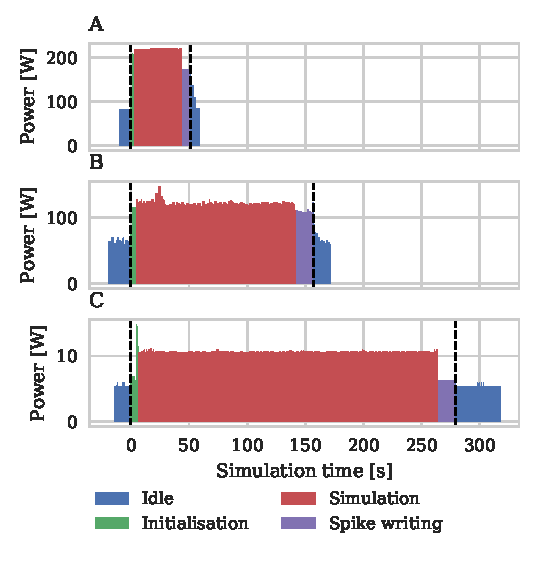
\includegraphics[width=85mm]{figures/microcircuit_power}
    \end{center}
    \caption{Power consumption during \SI{10}{\second} microcircuit simulation.
    Power was measured using consumer power measurement device with minimum resolution of \SI{0.1}{\watt} at mains socket.\\
    \textbf{(A)} Tesla K40c in a workstation with a Intel Xeon E5-1620 v2 processor running Ubuntu 16.04 LTS.\\
    \textbf{(B)} GeForce 1050Ti in a desktop PC with an Intel Core i5 750 processor running Windows 7.\\
    \textbf{(C)} NVIDIA Jetson TX2 development kit running Ubuntu 16.04 LTS in maximum performance mode. \todo{figure out JetPack version}}
    \label{fig:microcircuit_power}
\end{figure}

As well as recording the timings of the microcircuit benchmark described in the previous section, we also recorded the power usage of the systems being benchmarked using a consumer power measurement device at the mains socket.
The screen of the power measurement device was recorded using a webcam, optical character recognition was performed using `Seven Segment Optical Character Recognition' developed by \citet{Auerswald2018} and the resultant power measurements were tagged with a time and written to disk.
Figure~\ref{fig:microcircuit_power} shows the power usage over time for simulations of the microcircuit model running for \SI{10}{\second} of biological time on each of the devices listed in table~\ref{tab:gpu_devices} aside from the Tesla V100 which we do not have local access to record the power usage of the entire system.

\begin{table}
  \centering
  \begin{tabular}{r S S S}
    \toprule
        {Model}                 & {Energy to solution}      & {Simulation energy}       & {Energy per synaptic event} \\
                                & {[\si{\kilo\watt\hour}]}  & {[\si{\kilo\watt\hour}]}  & {[\si{\micro\joule}]} \\
    \midrule
        GeForce 1050 Ti         & 0.0053                    & 0.0051                    & 2.0 \\
        Jetson TX2              & 0.00080                   & 0.00078                   & 0.30  \\
        Tesla K40c              & 0.0030                    & 0.0028                    & 1.08 \\
        SpiNNaker               & {--}                      & 0.017                     & 5.9 \textsuperscript{1}\\
        NEST (lowest energy)    & {--}                      & 0.012                     & 4.4 \\
    \bottomrule
  \end{tabular}

  \caption{Energy cost of simulations.
  Energy to solution and simulation energy of GPU are calculated using the \lstinline{numpy.trapz} and the simulation energy is divided by the total number of synaptic events processed to obtain the energy per synaptic event.
  For comparison, simulation energies for SpiNNaker and the NEST simulation with the lowest simulation energy (2 nodes)are read off the figure presented by \citet{VanAlbada2018}.
  Energies per synaptic event for SpiNNaker and the NEST are those reported by \citet{VanAlbada2018}.\\
  \textsuperscript{1}~This energy per synaptic event is calculated after the `idle' power of the SpiNNaker system has been taken into account.}
  \label{tab:energy_measures}
\end{table}

By integrating the power time series using the \lstinline{numpy.trapz} function we then calculated the energy to solution for each device as well as the energy per synaptic event -- a common measure for comparing the energy efficiency of neuromorphic systems.
These energy costs are listed in table~\ref{tab:energy_measures} alongside the energy costs presented by \citet{VanAlbada2018} for simulations running onn SpiNNaker and a CPU-based cluster.

From figure~\ref{fig:microcircuit_power} we can see that even an idling workstation draws on the order of \SI{100}{\watt} and, as \citeauthor{VanAlbada2018} discusses, a single infiniband switch has a TDP of over \SI{200}{\watt}.
Therefore it is somewhat unsurprising that any accelator that allows equivalent simulations to be run on fewer nodes would significantly improve energy usage.
Furthermore, as \citeauthor{VanAlbada2018} discusses, slowing SpiNNaker simulations down to this degree and simulating so few neurons on each processor results in very poor energy efficiency.
However, in a previous study using a much smaller cortical microcircuit model suffering from none of these issues, \citet{Sharp2012} measured the power usage of a SpiNNaker system energy usage corresponded to \SI{0.11}{\micro\joule} per synaptic event.
This suggests that through 

Whilst we were unable to measure the energy of the Tesla V100 system directly, Tesla GPUs have built in power monitoring which shows that the Tesla V100 drew a maximum of \SI{88}{\watt} compared to \SI{107}{\watt} for the Tesla K40c.
As the workstation containing the Tesla K40c drew \SI{218}{\watt} while simulating the model, compared to an idle power draw of \SI{84}{\watt}, we can estimate that the single CPU core being used by the simulation was drawing \SI{27}{\watt} more than when the system was idle.
Therefore we can estimate that, if a Tesla V100 was attached to the same workstation, the maximum power draw would be reduced to \SI{199}{\watt} meaning that, based on the reduced simulation time of \SI{22}{\second}, the simulation energy for such a system would be \SI{0.0012}{\kilo\watt\hour} and the energy per synaptic event would be \SI{0.47}{\micro\joule}.

\section{Discussion}
\begin{itemize}
    \item Fewer nodes with more specialised accelerators are the only route to lower power HPC simulations.
\end{itemize}

\subsection{Neurorobotics}
afa

\subsection{Interactive simulation}
asfs

\subsection{Further optimisation and GPU architectures}

Because the SIMT programming model used by GPUs does not require the complex coherant caches which is making simply adding more CPU cores to symmetric multiprocessing difficult~\todo{citation}, it is expected that GPU hardware will continue to scale~ \todo{citation}.
However, even with new even higher speed memory technologies such as HBM3~\todo{citation}, memory bandwidth has historically always lagged behind processing performance.


\begin{itemize}
    \item Half precision float, ILP - should double performance on TX1
\end{itemize}

\begin{itemize}
    \item HBM3 - further doubling of memory bandwidth
    \item FP16 - half memory bandwidth, double arithmetic throughput
\end{itemize}

\section*{Conflict of Interest Statement}
The authors declare that the research was conducted in the absence of any commercial or financial relationships that could be construed as a potential conflict of interest.

\section*{Author Contributions}
The Author Contributions section is mandatory for all articles, including articles by sole authors. If an appropriate statement is not provided on submission, a standard one will be inserted during the production process. The Author Contributions statement must describe the contributions of individual authors referred to by their initials and, in doing so, all authors agree to be accountable for the content of the work. Please see  \href{http://home.frontiersin.org/about/author-guidelines#AuthorandContributors}{here} for full authorship criteria.

\section*{Funding}
Details of all funding sources should be provided, including grant numbers if applicable. Please ensure to add all necessary funding information, as after publication this is no longer possible.

\section*{Acknowledgments}
We would like to thank Andrew Webb for his thoughts on efficient parallel connectivity generation.
We would also like to thank Sacha van Albada for providing the data from her NEST simulations and clarifying some parts of the accuracy analysis -- without these contributions section~\ref{sec:results/correctness} would not have been possible.
This is a short text to acknowledge the contributions of specific colleagues, institutions, or agencies that aided the efforts of the authors.

\section*{Data Availability Statement}
The datasets [GENERATED/ANALYZED] for this study can be found in the [NAME OF REPOSITORY] [LINK].
% Please see the availability of data guidelines for more information, at https://www.frontiersin.org/about/author-guidelines#AvailabilityofData
%
\bibliographystyle{frontiersinSCNS_ENG_HUMS}
\bibliography{frontiers_genn}

%%% Make sure to upload the bib file along with the tex file and PDF
%%% Please see the test.bib file for some examples of references

\end{document}
